\subsection{DC モータサーボのカスケード制御と電流・電圧限界}

目標値の整形とレート制限を入れると、位置指令や速度指令は急な段差を持たなくなる。それでも、アクチュエータが実際に出せる電流、電圧、トルクには上限がある。ここでは、軸の位置を合わせる DC モータサーボを使い、電圧が電流を作り、電流がトルクを作り、トルクが速度と位置を変えるという物理の順序に沿って、電流ループ、速度ループ、位置ループを分ける。

直前までの PID とアンチワインドアップでは、計算入力 $u_c$ と印加入力 $u$ の差を一つの飽和器として扱った。DC モータでは、その飽和器の内側に少なくとも二つの制約がある。一つは巻線・インバータ・電源で決まる電流上限、もう一つは逆起電力と抵抗降下を含む電圧上限である。これらを分けて見ないと、外側の位置制御器が「もっと大きなトルクを出せば速く追従できる」と計算していても、内側の電流ループが実現できない理由を説明できない。

\subsubsection{DC モータで分かれる三つの信号}

剛体軸に接続された DC モータを、次の単純化モデルで扱う。
\begin{align}
  L\dot{i}+Ri+K_e\omega&=v,\\
  J\dot{\omega}+b\omega&=K_t i-\tau_L,\\
  \dot{\theta}&=\omega.
  \label{eq:cascade-dc-motor}
\end{align}
$v$ は端子電圧 $[\mathrm{V}]$、$i$ は電機子電流 $[\mathrm{A}]$、$\tau_m=K_t i$ はモータトルク $[\mathrm{N\,m}]$、$\omega$ は角速度 $[\mathrm{rad/s}]$、$\theta$ は角度 $[\mathrm{rad}]$ である。$R[\Omega]$、$L[\mathrm{H}]$、$K_e[\mathrm{V\,s/rad}]$、$K_t[\mathrm{N\,m/A}]$、$J[\mathrm{kg\,m^2}]$、$b[\mathrm{N\,m\,s/rad}]$ は正の定数とする。ここではクーロン摩擦、デッドゾーン、バックラッシュは入れない。これらは電流・電圧制約の後に残る別の実装限界として次に扱う。

電気式の左辺を見ると、電圧 $v$ は三つの成分に使われる。$L\dot{i}$ は電流を速く変えるための電圧、$Ri$ は巻線抵抗で消費される電圧、$K_e\omega$ は回転速度に比例する逆起電力である。したがって、同じ電流指令でも、低速でゆっくり変えるときと、高速で急に増やすときでは必要電圧が違う。機械式では、電流 $i$ がトルク $K_t i$ へ変換され、そのトルクから粘性抵抗 $b\omega$ と負荷トルク $\tau_L$ を差し引いたものが角加速度 $J\dot{\omega}$ を決める。

この信号の順序から、自然なカスケード構造は次の三段になる。
\begin{align}
  \text{位置ループ:}\quad
  \omega_r&=C_\theta(s)(\theta_r-\theta),\\
  \text{速度ループ:}\quad
  i_r^c&=C_\omega(s)(\omega_r-\omega),\\
  \text{電流ループ:}\quad
  v_c&=C_i(s)(i_r-i).
  \label{eq:cascade-loop-signals}
\end{align}
$\theta_r$ の単位は $[\mathrm{rad}]$、$\omega_r$ の単位は $[\mathrm{rad/s}]$、$i_r^c$ と $i_r$ の単位は $[\mathrm{A}]$、$v_c$ の単位は $[\mathrm{V}]$ である。速度ループの出力は、物理的には「出したいトルクを電流で表した量」である。電流ループの出力は、その電流を実現するための電圧指令である。

\begin{figure}[tbp]
\centering
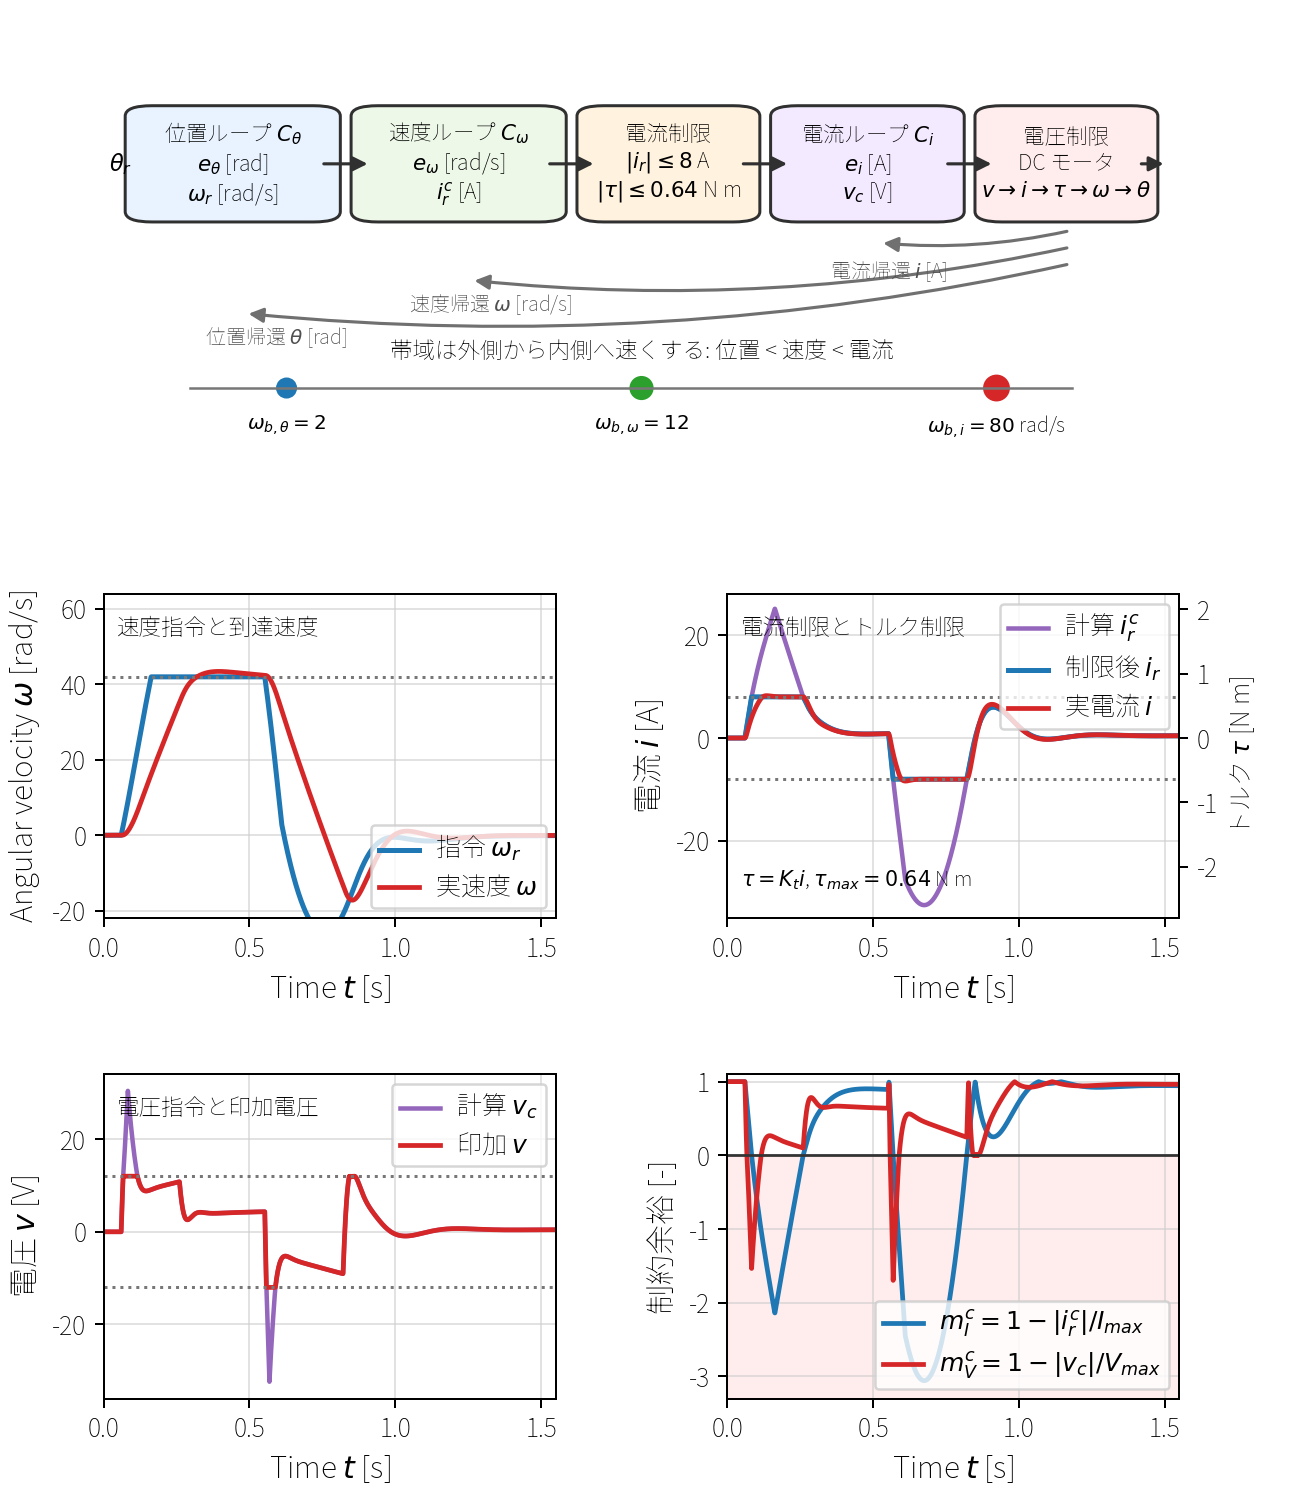
\includegraphics[width=0.98\linewidth,bb=0 0 1296 1512]{figures/cascade_actuator_limits_examples.png}
\caption{DC モータ位置サーボのカスケード構成と電流・電圧限界。上段は位置、速度、電流の三つのループを外側から内側へ配置し、帯域幅を $\omega_{b,\theta}=2\,\mathrm{rad/s}$、$\omega_{b,\omega}=12\,\mathrm{rad/s}$、$\omega_{b,i}=80\,\mathrm{rad/s}$ の順に速くした例である。下段は $R=1.0\,\Omega$、$L=0.050\,\mathrm{H}$、$K_t=K_e=0.08$、$J=0.003\,\mathrm{kg\,m^2}$、$b=0.002\,\mathrm{N\,m\,s/rad}$、$I_{\max}=8\,\mathrm{A}$、$V_{\max}=12\,\mathrm{V}$ としたシミュレーションで、速度指令、電流指令、印加電圧、制約余裕を同じ時間軸で示す。電流指令 $i_r^c$ と電圧指令 $v_c$ の余裕が 0 を下回る時間帯では、外側ループが要求したトルク変化を内側ループが実現できない。}
\label{fig:cascade-actuator-limits-examples}
\end{figure}

\wfig{cascade-actuator-limits-examples} の上段は、三つの信号をどのループが作るかを示している。位置制御器は速度指令を作るだけであり、直接電圧を決めない。速度制御器は電流指令を作るだけであり、直接位置を動かすわけではない。電流制御器だけが電圧を出し、その電圧がモータ巻線と逆起電力を通して実電流を変える。この分担を明確にすると、飽和がどの信号で起きたのかを分けて読める。

\subsubsection{帯域分離と等価対象}

内側電流ループが閉ループ伝達関数
\begin{equation}
  T_i(s)=\frac{I(s)}{I_r(s)}
\end{equation}
で表されるとする。外側の速度ループが使う周波数範囲で
\begin{equation}
  T_i(j\omega)\simeq 1,
  \qquad
  \angle T_i(j\omega)\simeq 0
  \quad (0\leq\omega\leq\omega_{b,\omega})
  \label{eq:current-loop-fast-condition}
\end{equation}
なら、速度ループから見ると $i\simeq i_r$ と近似できる。このとき \weq{cascade-dc-motor} の機械式は
\begin{align}
  J\dot{\omega}+b\omega
  &\simeq K_t i_r-\tau_L
\end{align}
であり、負荷トルクをいったん 0 とおくと、電流指令から速度までの等価対象は
\begin{equation}
  \frac{\Omega(s)}{I_r(s)}
  \simeq
  \frac{K_t}{Js+b}
  \label{eq:current-to-speed-equivalent}
\end{equation}
になる。さらに位置は $\dot{\theta}=\omega$ なので、
\begin{equation}
  \frac{\theta(s)}{I_r(s)}
  \simeq
  \frac{K_t}{s(Js+b)}
  \label{eq:current-to-position-equivalent}
\end{equation}
である。位置ループはこの二重の遅れを相手にするため、速度ループより遅く置く。

帯域幅を、位置ループ $\omega_{b,\theta}$、速度ループ $\omega_{b,\omega}$、電流ループ $\omega_{b,i}$ と書く。設計の目安は
\begin{equation}
  \omega_{b,i}\geq 5\omega_{b,\omega},
  \qquad
  \omega_{b,\omega}\geq 5\omega_{b,\theta}
  \label{eq:cascade-bandwidth-order}
\end{equation}
である。これは厳密な定理ではなく、外側ループが内側ループをほぼ比例要素として扱える範囲を確保するための実務的な条件である。\wfig{cascade-actuator-limits-examples} の上段では、$2$、$12$、$80\,\mathrm{rad/s}$ としてこの順序を示した。内側を速くしすぎると、電流測定ノイズ、PWM 遅れ、電圧飽和の影響が増えるため、帯域を上げるほどよいわけではない。

\subsubsection{電流・トルク・電圧・速度の限界}

速度ループが計算した電流指令を $i_r^c$ とする。インバータ、巻線温度、電源容量から連続または短時間の電流上限 $I_{\max}$ が決まると、電流ループに渡す指令は
\begin{equation}
  i_r=\operatorname{sat}_{[-I_{\max},I_{\max}]}(i_r^c)
  \label{eq:current-command-limit}
\end{equation}
である。トルクは $\tau_m=K_t i$ なので、電流制限は同時に
\begin{equation}
  |\tau_m|\leq K_t I_{\max}
  \label{eq:torque-current-limit}
\end{equation}
というトルク制限でもある。図の例では $I_{\max}=8\,\mathrm{A}$、$K_t=0.08\,\mathrm{N\,m/A}$ だから、到達できるトルクは $0.64\,\mathrm{N\,m}$ までである。速度ループが $i_r^c=15\,\mathrm{A}$ を計算しても、モータへは $8\,\mathrm{A}$ 相当のトルクしか要求できない。

一方、電流が制限内でも、電圧上限が先に効くことがある。\weq{cascade-dc-motor} の電気式を電圧について解くと
\begin{equation}
  v=L\dot{i}+Ri+K_e\omega
  \label{eq:voltage-required-current}
\end{equation}
である。電源電圧を $V_{\max}$ とすると、印加電圧は
\begin{equation}
  v=\operatorname{sat}_{[-V_{\max},V_{\max}]}(v_c)
  \label{eq:voltage-command-limit}
\end{equation}
になる。電流を速く増やしたいときは $L\dot{i}$ が大きくなり、高速回転中は $K_e\omega$ が大きくなる。したがって、低速では実現できた同じ電流指令が、高速では逆起電力のために実現できない場合がある。準定常で $\dot{i}\simeq0$ と見なせるなら、
\begin{equation}
  |Ri+K_e\omega|\leq V_{\max}
  \label{eq:steady-voltage-limit}
\end{equation}
が必要である。正転で正電流を流すときは、概略的に
\begin{equation}
  \omega\leq\frac{V_{\max}-Ri}{K_e}
  \label{eq:voltage-speed-current-limit}
\end{equation}
となり、速度が上がるほど同時に出せる電流、つまりトルクが小さくなる。

図の下段では、計算電流 $i_r^c$ は最初の加速区間で $I_{\max}$ を超えている。制限後の $i_r$ は $8\,\mathrm{A}$ で頭打ちになり、実電流 $i$ はさらに電圧上限と巻線時定数のために遅れて立ち上がる。電圧指令 $v_c$ は $V_{\max}=12\,\mathrm{V}$ を大きく超える時間帯があり、印加電圧 $v$ は上限に張り付く。制約余裕
\begin{equation}
  m_I^c=1-\frac{|i_r^c|}{I_{\max}},
  \qquad
  m_V^c=1-\frac{|v_c|}{V_{\max}}
  \label{eq:constraint-margin}
\end{equation}
は、計算指令が制約内なら正、制約ちょうどなら 0、実現不能なら負になる。余裕が負になっている時間帯では、外側ループの計算結果をそのまま物理入力として扱ってはいけない。

\subsubsection{電流ループ飽和時に崩れる前提}

カスケード制御の外側ループは、内側の電流ループが \weq{current-loop-fast-condition} を満たし、$i\simeq i_r$ になることを前提にしている。電圧飽和または電流制限に入ると、この前提が崩れる。実際の電流変化は
\begin{equation}
  \dot{i}
  =
  \frac{
  \operatorname{sat}_{[-V_{\max},V_{\max}]}(v_c)-Ri-K_e\omega
  }{L}
  \label{eq:saturated-current-dynamics}
\end{equation}
で決まり、制御器が計算した $v_c$ ではなく、飽和後の電圧でしか動かない。つまり、内側閉ループはもはや速い比例要素ではなく、電圧上限に張り付いた非線形な電流立上りになる。

このとき速度ループには、必要なトルクが出ていないことが速度偏差の残りとして現れる。速度ループや位置ループに積分器があると、その偏差を消そうとしてさらに大きな電流指令を蓄積し、外側のワインドアップを起こす。したがって、電流制限を入れるだけでは不十分であり、制限後の $i_r$ と実電流 $i$ の情報を外側のアンチワインドアップへ戻す必要がある。速度ループの積分状態を、$i_r^c-i_r$ または実トルク不足 $K_t(i_r-i)$ に応じて戻す構成にすると、外側ループは「トルクがまだ出ていない」ことを内部状態にも反映できる。

もう一つの失敗は帯域順序の見かけ上の崩れである。線形設計では $\omega_{b,i}$ が十分大きくても、飽和中の電流変化率は \weq{saturated-current-dynamics} の上限で決まる。電流が遅れている時間帯では、速度ループが期待した位相とゲインが得られない。位置ループは速度ループの遅れを、速度ループは電流ループの遅れを、それぞれ未知の対象遅れとして受け取るため、振動や行き過ぎが増える。

ここまでで、目標値を滑らかにしても、電流、トルク、電圧、速度の制約が実現可能な応答を決めることが分かった。次に残る限界は、制約内の小さな電圧やトルクを出しているにもかかわらず、静止摩擦、デッドゾーン、バックラッシュのために軸が思った通り動かない場合である。したがって、次の段階では、電流・電圧の上限ではなく、入力と運動の間にある不感帯と履歴を分けて扱う。
